\documentclass{beamer}
\usetheme{Copenhagen}
 
 
%Information to be included in the title page:
\title{Transporte TCP}
\author{Antunez Joaquin, Gonzalez Alejo y Nielsen Maximiliano}
\institute{Instituto Politécnico Superior Gral. San Martín}
\date{2019}
 
\begin{document}
 
\frame{\titlepage}
 
\begin{frame}
\frametitle{Conexiones TCP}
Las conexiones del protocolo TCP se podrían resumir en 3 pasos.
TCP es orientado a la conexión, es decir, que antes de las dos redes en cuestión se comuniquen y empiece la transferencia de datos se debe establecer una conexión.
\vspace{5mm}
\begin{enumerate}
\item Establecimiento de la conexión
\item Transferencia de datos
\item Liberación de la conexión
\end{enumerate}

\vspace{5mm}

El establecimiento de dicha conexión se realiza con el método three-way handshake y el cierre con el método four-way handshake.

\end{frame}

\begin{frame}
\frametitle{Establecimiento de la conexión}
3-way handshake (confirmación de 3 pasos): En este método el cliente y el servidor intercambian paquetes SYN y ACK antes de que la comunicación y transferencia de datos comience.
\vspace{5mm}
\begin{itemize}
\item SYN: Es utilizado para establecer conexiones. En esencia es usado para indicar REQUERIMIENTO DE CONEXIÓN y CONEXIÓN ACEPTADA.
\item ACK: Es igual a 1 para indicar que el número de reconocimiento es válido. Si vale 0, el paquete no contiene un reconocimiento, y entonces el campo número de reconocimiento es ignorado.
\end{itemize}
\end{frame}

\begin{frame}
\frametitle{Establecimiento de la conexión: 3-way handshake}
\begin{enumerate}
\item El cliente envía un paquete SYN hacia el servidor para averiguar si este está disponible para entablar nuevas conexiones.
\item El servidor, que tiene abiertos los puertos necesarios para que se puede iniciar una conexión, al recibir el paquete SYN del cliente le responde enviando una confirmación, un paquete SYN/ACK.
\item El cliente responde con un paquete de confirmación ACK.
\end{enumerate}
\end{frame}

\begin{frame}
\frametitle{Establecimiento de la conexión: 3-way handshake}
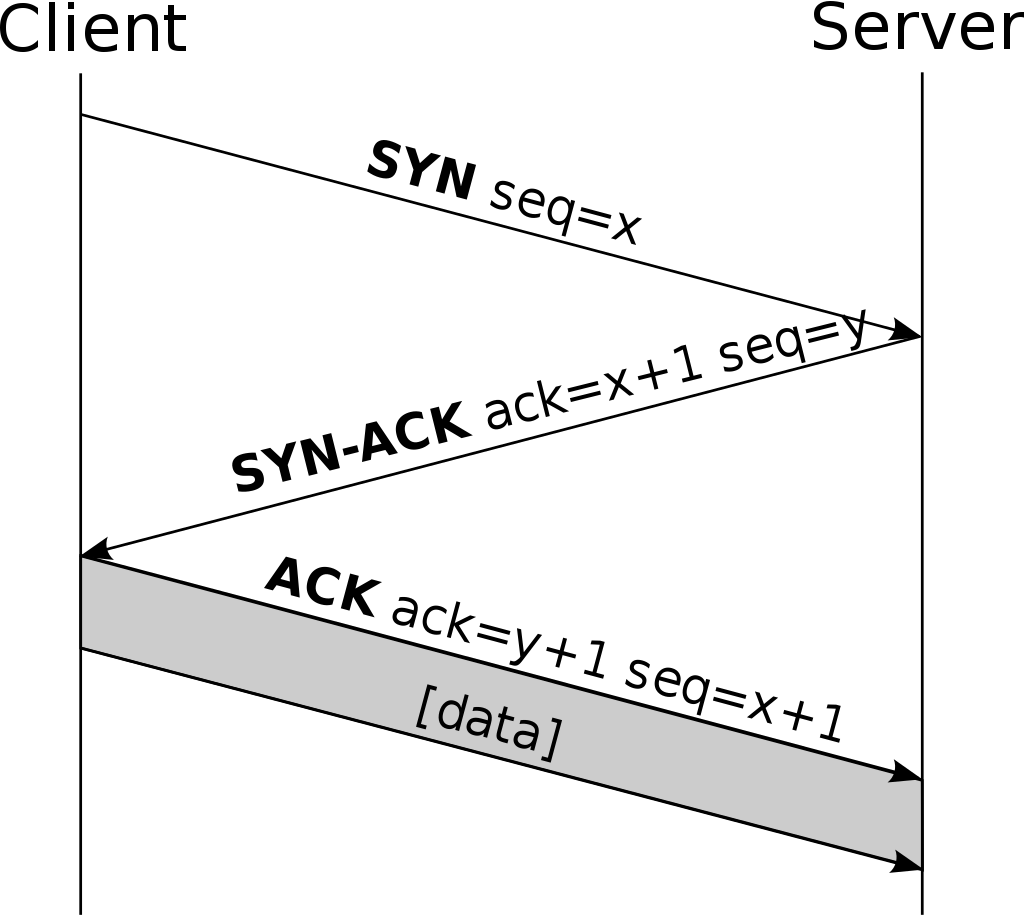
\includegraphics[scale=0.2]{3}\\
\vspace{5mm}
Una vez que este proceso concluye, las dos partes ya pueden iniciar la transferencia de datos.
\end{frame}

\begin{frame}
\frametitle{Transferencia de datos}
Segmento TCP: En el protocolo TCP (capa transporte) los datos se envían en forma de segmento.\\
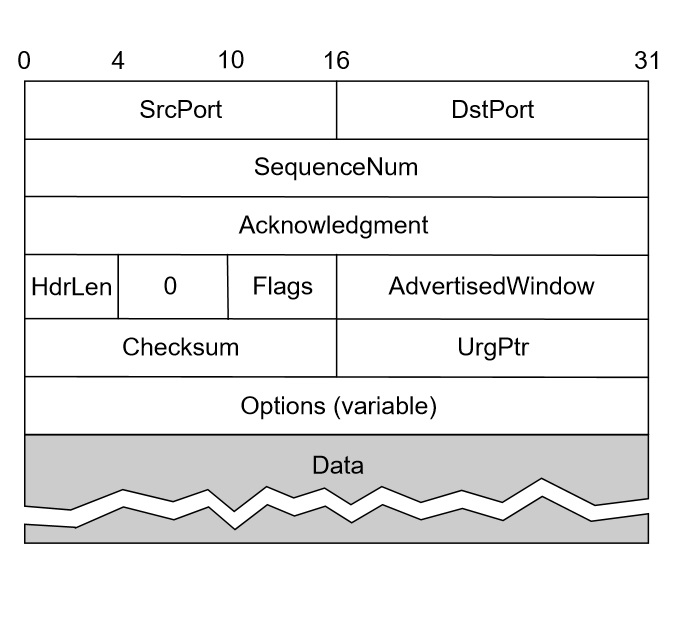
\includegraphics[scale=0.5]{segmento}\\
\end{frame}

\begin{frame}
\frametitle{Transferencia de datos: formato de segmento}
\begin{itemize}
\item Puerto fuente y puerto destino (16 bits) : Identifican los puntos finales locales de la conexión.
\item Número de Secuencia (32 bits): El cliente y servidor envían sus números de secuencia (nótese distintos) durante el establecimiento de la conexión, de manera que identifica de forma inequívoca los datos de aplicación que contiene el segmento TCP. Distingue el primer byte de datos.
\item Número de reconocimiento (32 bits) (si ACK es establecido) : El indica el siguiente byte que espera el receptor.
\item Longitud cabecera (4 bits):Indica cuántas palabras de 32 bits están contenidas en la cabecera de TCP. Es necesario a causa de la longitud variable del campo Opciones.
\end{itemize}
\end{frame}

\begin{frame}
\frametitle{Transferencia de datos: formato de segmento}
\begin{itemize}
\item Flags
\begin{itemize}
\item SYN
\item ACK
\item FIN
\item URG: Es igual a 1 si el campo Puntero a urgente está en uso. 
\item PSH: “PUSHed data”. Indica al receptor que debe entregar los datos a la aplicación inmediatamente después del arribo del paquete. No debe esperar hasta que un buffer total haya sido recibido.
\item RST: Se utiliza para resetear una conexión que se ha vuelto confusa debido a la caída de un host o alguna otra razón.
\end{itemize}
\item Tamaño de la ventana: Indica cuántos bytes pueden ser enviados comenzando desde el último byte reconocido. Para propósitos de control de flujo.
\item Suma de verificación (16 bits): Checksum utilizado para la comprobación de errores tanto en la cabecera como en los datos.
\end{itemize}
\end{frame}

\begin{frame}
\frametitle{Transferencia de datos: formato de segmento}
\begin{itemize}
\item Código de redundancia: Verifica la cabecera y los datos.
Puntero urgente (si URG es establecido): Se utiliza para indicar un desplazamiento en bytes a partir del número de secuencia actual en el que se encuentran los datos urgentes. Esta facilidad se brinda en lugar de los mensajes de interrupción.
\item Opciones: Diseñado para proveer una manera de adicionar facilidades extras no cubiertas por la cabecera regular.
\end{itemize}
\end{frame}

\begin{frame}
\frametitle{Liberación de la conexión}
4-way handshake (confirmación de 4 pasos): en este método el cliente y servidor intercambian paquetes FIN y ACK una vez que la transferencia de datos haya finalizado.
\vspace{5mm}
\begin{itemize}
\item FIN: Es utilizado para liberar conexiones. Especifica que el emisor no tiene más datos para transmitir. 
\end{itemize}
\end{frame}

\begin{frame}
\frametitle{Liberación de la conexión: 4-way handshake}
Pasos:
\vspace{5mm}
\begin{enumerate}
\item La parte que desee terminar su comunicación (generalmente el cliente) envía un paquete FIN para avisarle a la otra parte que desea concluir su comunicación.
\item La parte que recibe el paquete FIN envía un paquete ACK de confirmación.
\item Esa misma parte que envió el paquete ACK envía un paquete FIN para finiquitar su comunicación.
\item La otra parte le envía un paquete ACK de confirmación.
\end{enumerate}
\end{frame}

\begin{frame}
\frametitle{Liberación de la conexión:4-way handshake}
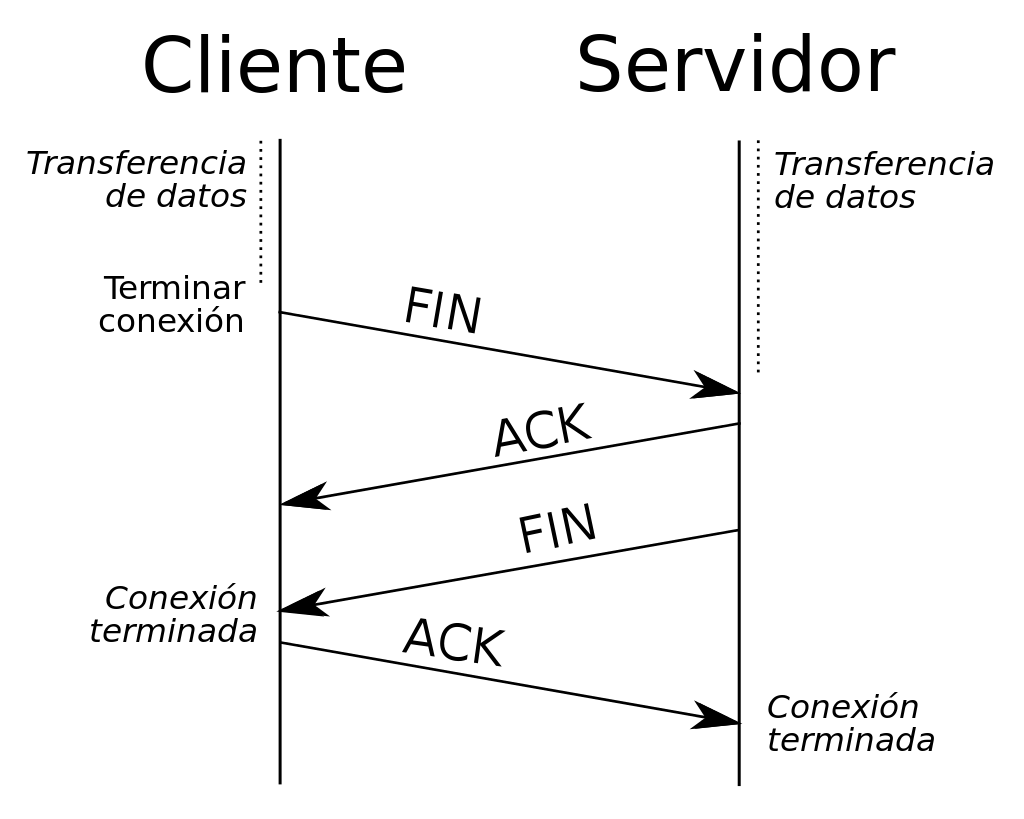
\includegraphics[scale=0.2]{4}\\
\end{frame}
\begin{frame}
	\frametitle{Ventana deslizante}
	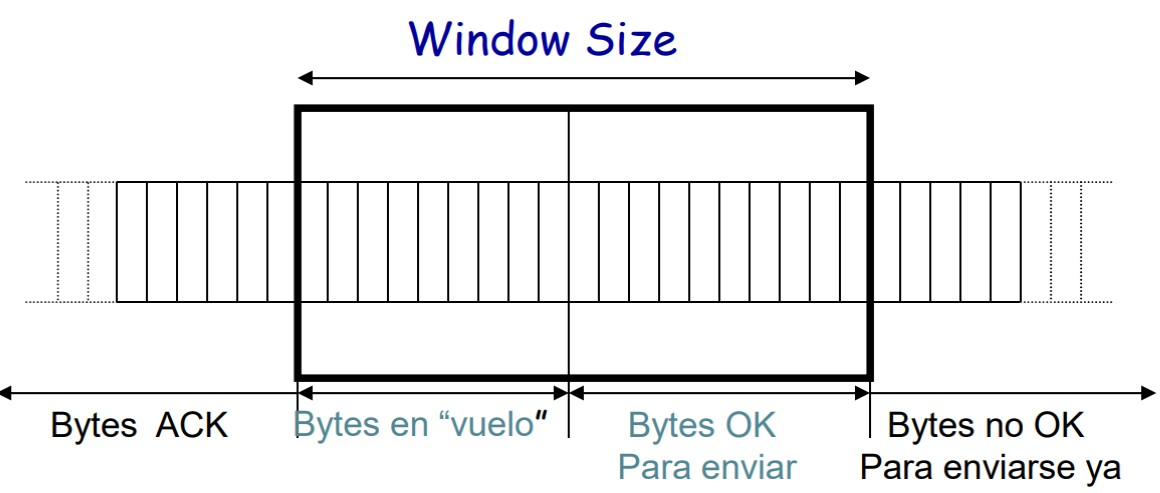
\includegraphics[width=\textwidth]{ventdesl}
	\begin{enumerate}
		\item Política de retransmisión “Go Back N”.
		\item window size es “advertised” por el receptor ( server)
		(usualmente 4k – 8k Bytes en connection set-up).
	\end{enumerate}
\end{frame}
\begin{frame}
	\frametitle{Ventana deslizante}
	TCP implementa una variante del protocolo de ventana deslizante. Este permite al emisor transmitir múltiples segmentos de información antes de comenzar la espera para que el receptor le confirme la recepción de los segmentos, tal confirmación se llama validación, y consiste en el envío de mensajes denominados ACK del receptor al emisor. \\
	Características del protocolo:\\
	\begin{enumerate}
		\item Garantiza Confiabilidad
		\item La aplicación recibe los datos en orden
		\item Fuerza el control de flujo entre receptor y transmisor
	\end{enumerate}
\end{frame}

\begin{frame}
	\frametitle{Ventana Deslizante comunicacíon}
	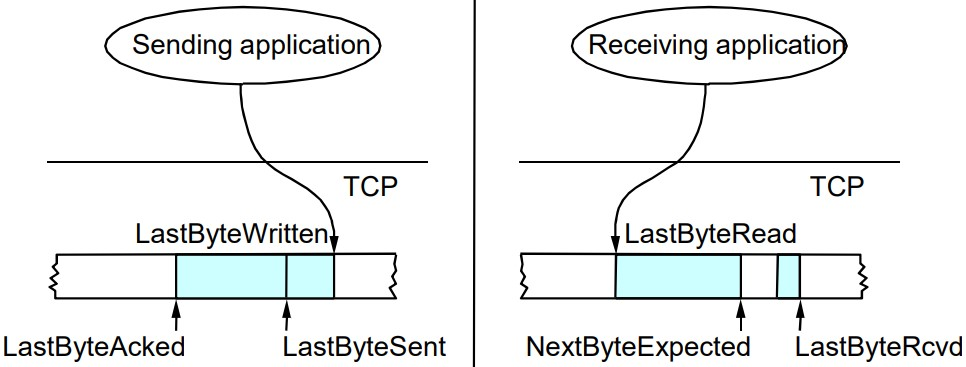
\includegraphics[width=\textwidth]{vdemisor}
\end{frame}
\begin{frame}
		\frametitle{Ventana Deslizante emisor}
	Lado del transmisor: Se encuentran 3 punteros, que siguen las siguientes relaciones:
	\begin{center}
\textbf{	LastByteAcked \textless= LastByteSent \\
	LastByteSent \textless= LastByteWritten}
	\end{center}
Se bufferean los bytes entre LastByteAcked ( los que están a su
derecha ya fueron confirmados) y LastByteWritten ( los que
están a su derecha no fueron generados …)
\end{frame}

\begin{frame}
		\frametitle{Ventana Deslizante receptor}
		Las relaciones son menos intuitivas debido al reordenamiento
		\begin{center}
			\textbf{LastByteRead \textless NextByteExpected}
		\end{center}
	Un byte no puede ser leído por la aplicación a menos que este se halla recibido y
	todos su
	precedentes.
	\begin{center}
	\textbf{	NextByteExpected \textless= LastByteRcvd +1}
	\end{center}
Si están en orden se cumple la igualdad . Si están en desorden
\textbf{NextByteExpected} apunta al espacio vacio antes de  \textbf{LastByteRead+1}.\\
Buffereamos los bytes entre \textbf{NextByteRead} y \textbf{LastByteRcvd}.
\end{frame}
 
 \begin{frame}
 		\frametitle{Ventana Deslizante Control de Flujo}
 		Tamaño del buffer de envío: \textbf{MaxSendBuffer}.\\
 		Tamaño del buffer de recepción: \textbf{MaxRcvBuffer}.\\
 		Lado receptor:
 		\begin{center}
 			\textbf{
 			LastByteRcvd - LastByteRead \textless= MaxRcvBuffer\\
 			 AdvertisedWindow = MaxRcvBuffer - (LastByteRcvd - NextByteRead)
 		}
 		\end{center}
 	Lado transmisor:
 	\begin{center}
 		\textbf{
 		LastByteSent - LastByteAcked  \textless= AdvertisedWindow\\
 		 EffectiveWindow = AdvertisedWindow - (LastByteSent - LastByteAcked)\\
 	 LastByteWritten - LastByteAcked \textless= MaxSendBuffer\\
 }\end{center}
 Bloquear Tx si (\textbf{LastByteWritten - LastByteAcked) + y \textless MaxSenderBuffer}, y
 bytes que se desean escribir.\\
 Siempre enviar ACK en respuesta a la llegada de segmentos. 
 Tx persiste enviando 1 byte cuando \textbf{AdvertisedWindow = 0} \\

 \end{frame}
 
\end{document}